\setchapterpreamble[u]{\margintoc}
\chapter{Is it an Algorithm or Machine Learning?}
\labch{intro}

\section{Algorithms: Codified Human Understanding}

AI is a shitty term

We tried a lot of things, teaching computers explicit grammar and explicit rules

IMO, this was not AI, this was codified human understanding.

In code, that understanding might look like this.... %(TODO GET CODIFIED LANGUAGE PROCESSOR)

TODO talk about this book \sidecite{Douthat2002}

\href{https://bradflaugher.com}{bradflaugher.com}.  
\sidenote{Snarky sidenote!} 


\section{Machine Learning: Data-Derived Insights}
\labsec{does}

Hardware got amazing, we gave up teaching the way we teach ourselves and let the data do the work

We leveraged huge statistical models to regress our way to success

We used building blocks of regression and neurons to train huge models

These models are statistical and deterministic, but ultimately chaotic black boxes..

TODO talk about these books \cite{MacAskill2022} \cite{Metz2022Sep} \cite{Metz2022Sep2} \cite{Aytekin}


\begin{marginfigure}[-5.5cm]
	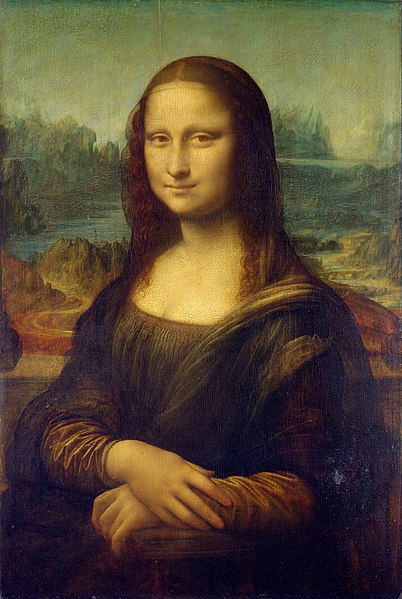
\includegraphics{monalisa}
	\caption[The Mona Lisa]{The Mona Lisa.\\ 
	\url{https://commons.wikimedia.org/wiki/File:Mona_Lisa,_by_Leonardo_da_Vinci,_from_C2RMF_retouched.jpg}}
	\labfig{marginmonalisa}
\end{marginfigure}
